\documentclass[11pt,fleqn]{book} % Default font size and left-justified equations

%%%%%%%%%%%%%%%%%%%%%%%%%%%%%%%%%%%%%%%%%
% The Legrand Orange Book
% Structural Definitions File
% Version 2.0 (9/2/15)
%
% Original author:
% Mathias Legrand (legrand.mathias@gmail.com) with modifications by:
% Vel (vel@latextemplates.com)
% 
% This file has been downloaded from:
% http://www.LaTeXTemplates.com
%
% License:
% CC BY-NC-SA 3.0 (http://creativecommons.org/licenses/by-nc-sa/3.0/)
%
%%%%%%%%%%%%%%%%%%%%%%%%%%%%%%%%%%%%%%%%%

%----------------------------------------------------------------------------------------
%	VARIOUS REQUIRED PACKAGES AND CONFIGURATIONS
%----------------------------------------------------------------------------------------

\usepackage[top=3cm,bottom=3cm,left=3cm,right=3cm,headsep=10pt,a4paper]{geometry} % Page margins

\usepackage{graphicx} % Required for including pictures
\graphicspath{{Pictures/}} % Specifies the directory where pictures are stored

\usepackage{lipsum} % Inserts dummy text

\usepackage{tikz} % Required for drawing custom shapes

\usepackage[english]{babel} % English language/hyphenation

\usepackage{enumitem} % Customize lists
\setlist{nolistsep} % Reduce spacing between bullet points and numbered lists

\usepackage{booktabs} % Required for nicer horizontal rules in tables

\usepackage{xcolor} % Required for specifying colors by name
\definecolor{ocre}{RGB}{243,102,25} % Define the orange color used for highlighting throughout the book

%----------------------------------------------------------------------------------------
%	FONTS
%----------------------------------------------------------------------------------------

\usepackage{avant} % Use the Avantgarde font for headings
%\usepackage{times} % Use the Times font for headings
\usepackage{mathptmx} % Use the Adobe Times Roman as the default text font together with math symbols from the Sym­bol, Chancery and Com­puter Modern fonts

\usepackage{microtype} % Slightly tweak font spacing for aesthetics
\usepackage[utf8]{inputenc} % Required for including letters with accents
\usepackage[T1]{fontenc} % Use 8-bit encoding that has 256 glyphs

%----------------------------------------------------------------------------------------
%	BIBLIOGRAPHY AND INDEX
%----------------------------------------------------------------------------------------

\usepackage[style=alphabetic,citestyle=numeric,sorting=nyt,sortcites=true,autopunct=true,babel=hyphen,hyperref=true,abbreviate=false,backref=true,backend=biber]{biblatex}
\addbibresource{bibliography.bib} % BibTeX bibliography file
\defbibheading{bibempty}{}

\usepackage{calc} % For simpler calculation - used for spacing the index letter headings correctly
\usepackage{makeidx} % Required to make an index
\makeindex % Tells LaTeX to create the files required for indexing

%----------------------------------------------------------------------------------------
%	MAIN TABLE OF CONTENTS
%----------------------------------------------------------------------------------------

\usepackage{titletoc} % Required for manipulating the table of contents

\contentsmargin{0cm} % Removes the default margin

% Part text styling
\titlecontents{part}[0cm]
{\addvspace{20pt}\centering\large\bfseries}
{}
{}
{}

% Chapter text styling
\titlecontents{chapter}[1.25cm] % Indentation
{\addvspace{12pt}\large\sffamily\bfseries} % Spacing and font options for chapters
{\color{ocre!60}\contentslabel[\Large\thecontentslabel]{1.25cm}\color{ocre}} % Chapter number
{\color{ocre}}  
{\color{ocre!60}\normalsize\;\titlerule*[.5pc]{.}\;\thecontentspage} % Page number

% Section text styling
\titlecontents{section}[1.25cm] % Indentation
{\addvspace{3pt}\sffamily\bfseries} % Spacing and font options for sections
{\contentslabel[\thecontentslabel]{1.25cm}} % Section number
{}
{\hfill\color{black}\thecontentspage} % Page number
[]

% Subsection text styling
\titlecontents{subsection}[1.25cm] % Indentation
{\addvspace{1pt}\sffamily\small} % Spacing and font options for subsections
{\contentslabel[\thecontentslabel]{1.25cm}} % Subsection number
{}
{\ \titlerule*[.5pc]{.}\;\thecontentspage} % Page number
[]

% List of figures
\titlecontents{figure}[0em]
{\addvspace{-5pt}\sffamily}
{\thecontentslabel\hspace*{1em}}
{}
{\ \titlerule*[.5pc]{.}\;\thecontentspage}
[]

% List of tables
\titlecontents{table}[0em]
{\addvspace{-5pt}\sffamily}
{\thecontentslabel\hspace*{1em}}
{}
{\ \titlerule*[.5pc]{.}\;\thecontentspage}
[]

%----------------------------------------------------------------------------------------
%	MINI TABLE OF CONTENTS IN PART HEADS
%----------------------------------------------------------------------------------------

% Chapter text styling
\titlecontents{lchapter}[0em] % Indenting
{\addvspace{15pt}\large\sffamily\bfseries} % Spacing and font options for chapters
{\color{ocre}\contentslabel[\Large\thecontentslabel]{1.25cm}\color{ocre}} % Chapter number
{}  
{\color{ocre}\normalsize\sffamily\bfseries\;\titlerule*[.5pc]{.}\;\thecontentspage} % Page number

% Section text styling
\titlecontents{lsection}[0em] % Indenting
{\sffamily\small} % Spacing and font options for sections
{\contentslabel[\thecontentslabel]{1.25cm}} % Section number
{}
{}

% Subsection text styling
\titlecontents{lsubsection}[.5em] % Indentation
{\normalfont\footnotesize\sffamily} % Font settings
{}
{}
{}

%----------------------------------------------------------------------------------------
%	PAGE HEADERS
%----------------------------------------------------------------------------------------

\usepackage{fancyhdr} % Required for header and footer configuration

\pagestyle{fancy}
\renewcommand{\chaptermark}[1]{\markboth{\sffamily\normalsize\bfseries\chaptername\ \thechapter.\ #1}{}} % Chapter text font settings
\renewcommand{\sectionmark}[1]{\markright{\sffamily\normalsize\thesection\hspace{5pt}#1}{}} % Section text font settings
\fancyhf{} \fancyhead[LE,RO]{\sffamily\normalsize\thepage} % Font setting for the page number in the header
\fancyhead[LO]{\rightmark} % Print the nearest section name on the left side of odd pages
\fancyhead[RE]{\leftmark} % Print the current chapter name on the right side of even pages
\renewcommand{\headrulewidth}{0.5pt} % Width of the rule under the header
\addtolength{\headheight}{2.5pt} % Increase the spacing around the header slightly
\renewcommand{\footrulewidth}{0pt} % Removes the rule in the footer
\fancypagestyle{plain}{\fancyhead{}\renewcommand{\headrulewidth}{0pt}} % Style for when a plain pagestyle is specified

% Removes the header from odd empty pages at the end of chapters
\makeatletter
\renewcommand{\cleardoublepage}{
\clearpage\ifodd\c@page\else
\hbox{}
\vspace*{\fill}
\thispagestyle{empty}
\newpage
\fi}

%----------------------------------------------------------------------------------------
%	THEOREM STYLES
%----------------------------------------------------------------------------------------

\usepackage{amsmath,amsfonts,amssymb,amsthm} % For math equations, theorems, symbols, etc

\newcommand{\intoo}[2]{\mathopen{]}#1\,;#2\mathclose{[}}
\newcommand{\ud}{\mathop{\mathrm{{}d}}\mathopen{}}
\newcommand{\intff}[2]{\mathopen{[}#1\,;#2\mathclose{]}}
\newtheorem{notation}{Notation}[chapter]

% Boxed/framed environments
\newtheoremstyle{ocrenumbox}% % Theorem style name
{0pt}% Space above
{0pt}% Space below
{\normalfont}% % Body font
{}% Indent amount
{\small\bf\sffamily\color{ocre}}% % Theorem head font
{\;}% Punctuation after theorem head
{0.25em}% Space after theorem head
{\small\sffamily\color{ocre}\thmname{#1}\nobreakspace\thmnumber{\@ifnotempty{#1}{}\@upn{#2}}% Theorem text (e.g. Theorem 2.1)
\thmnote{\nobreakspace\the\thm@notefont\sffamily\bfseries\color{black}---\nobreakspace#3.}} % Optional theorem note
\renewcommand{\qedsymbol}{$\blacksquare$}% Optional qed square

\newtheoremstyle{blacknumex}% Theorem style name
{5pt}% Space above
{5pt}% Space below
{\normalfont}% Body font
{} % Indent amount
{\small\bf\sffamily}% Theorem head font
{\;}% Punctuation after theorem head
{0.25em}% Space after theorem head
{\small\sffamily{\tiny\ensuremath{\blacksquare}}\nobreakspace\thmname{#1}\nobreakspace\thmnumber{\@ifnotempty{#1}{}\@upn{#2}}% Theorem text (e.g. Theorem 2.1)
\thmnote{\nobreakspace\the\thm@notefont\sffamily\bfseries---\nobreakspace#3.}}% Optional theorem note

\newtheoremstyle{blacknumbox} % Theorem style name
{0pt}% Space above
{0pt}% Space below
{\normalfont}% Body font
{}% Indent amount
{\small\bf\sffamily}% Theorem head font
{\;}% Punctuation after theorem head
{0.25em}% Space after theorem head
{\small\sffamily\thmname{#1}\nobreakspace\thmnumber{\@ifnotempty{#1}{}\@upn{#2}}% Theorem text (e.g. Theorem 2.1)
\thmnote{\nobreakspace\the\thm@notefont\sffamily\bfseries---\nobreakspace#3.}}% Optional theorem note

% Non-boxed/non-framed environments
\newtheoremstyle{ocrenum}% % Theorem style name
{5pt}% Space above
{5pt}% Space below
{\normalfont}% % Body font
{}% Indent amount
{\small\bf\sffamily\color{ocre}}% % Theorem head font
{\;}% Punctuation after theorem head
{0.25em}% Space after theorem head
{\small\sffamily\color{ocre}\thmname{#1}\nobreakspace\thmnumber{\@ifnotempty{#1}{}\@upn{#2}}% Theorem text (e.g. Theorem 2.1)
\thmnote{\nobreakspace\the\thm@notefont\sffamily\bfseries\color{black}---\nobreakspace#3.}} % Optional theorem note
\renewcommand{\qedsymbol}{$\blacksquare$}% Optional qed square
\makeatother

% Defines the theorem text style for each type of theorem to one of the three styles above
\newcounter{dummy} 
\numberwithin{dummy}{section}
\theoremstyle{ocrenumbox}
\newtheorem{theoremeT}[dummy]{Theorem}
\newtheorem{problem}{Problem}[chapter]
\newtheorem{exerciseT}{Exercise}[chapter]
\theoremstyle{blacknumex}
\newtheorem{exampleT}{Example}[chapter]
\theoremstyle{blacknumbox}
\newtheorem{vocabulary}{Vocabulary}[chapter]
\newtheorem{definitionT}{Definition}[section]
\newtheorem{corollaryT}[dummy]{Corollary}
\theoremstyle{ocrenum}
\newtheorem{proposition}[dummy]{Proposition}

%----------------------------------------------------------------------------------------
%	DEFINITION OF COLORED BOXES
%----------------------------------------------------------------------------------------

\RequirePackage[framemethod=default]{mdframed} % Required for creating the theorem, definition, exercise and corollary boxes

% Theorem box
\newmdenv[skipabove=7pt,
skipbelow=7pt,
backgroundcolor=black!5,
linecolor=ocre,
innerleftmargin=5pt,
innerrightmargin=5pt,
innertopmargin=5pt,
leftmargin=0cm,
rightmargin=0cm,
innerbottommargin=5pt]{tBox}

% Exercise box	  
\newmdenv[skipabove=7pt,
skipbelow=7pt,
rightline=false,
leftline=true,
topline=false,
bottomline=false,
backgroundcolor=ocre!10,
linecolor=ocre,
innerleftmargin=5pt,
innerrightmargin=5pt,
innertopmargin=5pt,
innerbottommargin=5pt,
leftmargin=0cm,
rightmargin=0cm,
linewidth=4pt]{eBox}	

% Definition box
\newmdenv[skipabove=7pt,
skipbelow=7pt,
rightline=false,
leftline=true,
topline=false,
bottomline=false,
linecolor=ocre,
innerleftmargin=5pt,
innerrightmargin=5pt,
innertopmargin=0pt,
leftmargin=0cm,
rightmargin=0cm,
linewidth=4pt,
innerbottommargin=0pt]{dBox}	

% Corollary box
\newmdenv[skipabove=7pt,
skipbelow=7pt,
rightline=false,
leftline=true,
topline=false,
bottomline=false,
linecolor=gray,
backgroundcolor=black!5,
innerleftmargin=5pt,
innerrightmargin=5pt,
innertopmargin=5pt,
leftmargin=0cm,
rightmargin=0cm,
linewidth=4pt,
innerbottommargin=5pt]{cBox}

% Creates an environment for each type of theorem and assigns it a theorem text style from the "Theorem Styles" section above and a colored box from above
\newenvironment{theorem}{\begin{tBox}\begin{theoremeT}}{\end{theoremeT}\end{tBox}}
\newenvironment{exercise}{\begin{eBox}\begin{exerciseT}}{\hfill{\color{ocre}\tiny\ensuremath{\blacksquare}}\end{exerciseT}\end{eBox}}				  
\newenvironment{definition}{\begin{dBox}\begin{definitionT}}{\end{definitionT}\end{dBox}}	
\newenvironment{example}{\begin{exampleT}}{\hfill{\tiny\ensuremath{\blacksquare}}\end{exampleT}}		
\newenvironment{corollary}{\begin{cBox}\begin{corollaryT}}{\end{corollaryT}\end{cBox}}	

%----------------------------------------------------------------------------------------
%	REMARK ENVIRONMENT
%----------------------------------------------------------------------------------------

\newenvironment{remark}{\par\vspace{10pt}\small % Vertical white space above the remark and smaller font size
\begin{list}{}{
\leftmargin=35pt % Indentation on the left
\rightmargin=25pt}\item\ignorespaces % Indentation on the right
\makebox[-2.5pt]{\begin{tikzpicture}[overlay]
\node[draw=ocre!60,line width=1pt,circle,fill=ocre!25,font=\sffamily\bfseries,inner sep=2pt,outer sep=0pt] at (-15pt,0pt){\textcolor{ocre}{R}};\end{tikzpicture}} % Orange R in a circle
\advance\baselineskip -1pt}{\end{list}\vskip5pt} % Tighter line spacing and white space after remark

%----------------------------------------------------------------------------------------
%	SECTION NUMBERING IN THE MARGIN
%----------------------------------------------------------------------------------------

\makeatletter
\renewcommand{\@seccntformat}[1]{\llap{\textcolor{ocre}{\csname the#1\endcsname}\hspace{1em}}}                    
\renewcommand{\section}{\@startsection{section}{1}{\z@}
{-4ex \@plus -1ex \@minus -.4ex}
{1ex \@plus.2ex }
{\normalfont\large\sffamily\bfseries}}
\renewcommand{\subsection}{\@startsection {subsection}{2}{\z@}
{-3ex \@plus -0.1ex \@minus -.4ex}
{0.5ex \@plus.2ex }
{\normalfont\sffamily\bfseries}}
\renewcommand{\subsubsection}{\@startsection {subsubsection}{3}{\z@}
{-2ex \@plus -0.1ex \@minus -.2ex}
{.2ex \@plus.2ex }
{\normalfont\small\sffamily\bfseries}}                        
\renewcommand\paragraph{\@startsection{paragraph}{4}{\z@}
{-2ex \@plus-.2ex \@minus .2ex}
{.1ex}
{\normalfont\small\sffamily\bfseries}}

%----------------------------------------------------------------------------------------
%	PART HEADINGS
%----------------------------------------------------------------------------------------

% numbered part in the table of contents
\newcommand{\@mypartnumtocformat}[2]{%
\setlength\fboxsep{0pt}%
\noindent\colorbox{ocre!20}{\strut\parbox[c][.7cm]{\ecart}{\color{ocre!70}\Large\sffamily\bfseries\centering#1}}\hskip\esp\colorbox{ocre!40}{\strut\parbox[c][.7cm]{\linewidth-\ecart-\esp}{\Large\sffamily\centering#2}}}%
%%%%%%%%%%%%%%%%%%%%%%%%%%%%%%%%%%
% unnumbered part in the table of contents
\newcommand{\@myparttocformat}[1]{%
\setlength\fboxsep{0pt}%
\noindent\colorbox{ocre!40}{\strut\parbox[c][.7cm]{\linewidth}{\Large\sffamily\centering#1}}}%
%%%%%%%%%%%%%%%%%%%%%%%%%%%%%%%%%%
\newlength\esp
\setlength\esp{4pt}
\newlength\ecart
\setlength\ecart{1.2cm-\esp}
\newcommand{\thepartimage}{}%
\newcommand{\partimage}[1]{\renewcommand{\thepartimage}{#1}}%
\def\@part[#1]#2{%
\ifnum \c@secnumdepth >-2\relax%
\refstepcounter{part}%
\addcontentsline{toc}{part}{\texorpdfstring{\protect\@mypartnumtocformat{\thepart}{#1}}{\partname~\thepart\ ---\ #1}}
\else%
\addcontentsline{toc}{part}{\texorpdfstring{\protect\@myparttocformat{#1}}{#1}}%
\fi%
\startcontents%
\markboth{}{}%
{\thispagestyle{empty}%
\begin{tikzpicture}[remember picture,overlay]%
\node at (current page.north west){\begin{tikzpicture}[remember picture,overlay]%	
\fill[ocre!20](0cm,0cm) rectangle (\paperwidth,-\paperheight);
\node[anchor=north] at (4cm,-3.25cm){\color{ocre!40}\fontsize{220}{100}\sffamily\bfseries\@Roman\c@part}; 
\node[anchor=south east] at (\paperwidth-1cm,-\paperheight+1cm){\parbox[t][][t]{8.5cm}{
\printcontents{l}{0}{\setcounter{tocdepth}{1}}%
}};
\node[anchor=north east] at (\paperwidth-1.5cm,-3.25cm){\parbox[t][][t]{15cm}{\strut\raggedleft\color{white}\fontsize{30}{30}\sffamily\bfseries#2}};
\end{tikzpicture}};
\end{tikzpicture}}%
\@endpart}
\def\@spart#1{%
\startcontents%
\phantomsection
{\thispagestyle{empty}%
\begin{tikzpicture}[remember picture,overlay]%
\node at (current page.north west){\begin{tikzpicture}[remember picture,overlay]%	
\fill[ocre!20](0cm,0cm) rectangle (\paperwidth,-\paperheight);
\node[anchor=north east] at (\paperwidth-1.5cm,-3.25cm){\parbox[t][][t]{15cm}{\strut\raggedleft\color{white}\fontsize{30}{30}\sffamily\bfseries#1}};
\end{tikzpicture}};
\end{tikzpicture}}
\addcontentsline{toc}{part}{\texorpdfstring{%
\setlength\fboxsep{0pt}%
\noindent\protect\colorbox{ocre!40}{\strut\protect\parbox[c][.7cm]{\linewidth}{\Large\sffamily\protect\centering #1\quad\mbox{}}}}{#1}}%
\@endpart}
\def\@endpart{\vfil\newpage
\if@twoside
\if@openright
\null
\thispagestyle{empty}%
\newpage
\fi
\fi
\if@tempswa
\twocolumn
\fi}

%----------------------------------------------------------------------------------------
%	CHAPTER HEADINGS
%----------------------------------------------------------------------------------------

% A switch to conditionally include a picture, implemented by  Christian Hupfer
\newif\ifusechapterimage
\usechapterimagetrue
\newcommand{\thechapterimage}{}%
\newcommand{\chapterimage}[1]{\ifusechapterimage\renewcommand{\thechapterimage}{#1}\fi}%
\def\@makechapterhead#1{%
{\parindent \z@ \raggedright \normalfont
\ifnum \c@secnumdepth >\m@ne
\if@mainmatter
\begin{tikzpicture}[remember picture,overlay]
\node at (current page.north west)
{\begin{tikzpicture}[remember picture,overlay]
\node[anchor=north west,inner sep=0pt] at (0,0) {\ifusechapterimage\includegraphics[width=\paperwidth]{\thechapterimage}\fi};
\draw[anchor=west] (\Gm@lmargin,-9cm) node [line width=2pt,rounded corners=15pt,draw=ocre,fill=white,fill opacity=0.5,inner sep=15pt]{\strut\makebox[22cm]{}};
\draw[anchor=west] (\Gm@lmargin+.3cm,-9cm) node {\huge\sffamily\bfseries\color{black}\thechapter. #1\strut};
\end{tikzpicture}};
\end{tikzpicture}
\else
\begin{tikzpicture}[remember picture,overlay]
\node at (current page.north west)
{\begin{tikzpicture}[remember picture,overlay]
\node[anchor=north west,inner sep=0pt] at (0,0) {\ifusechapterimage\includegraphics[width=\paperwidth]{\thechapterimage}\fi};
\draw[anchor=west] (\Gm@lmargin,-9cm) node [line width=2pt,rounded corners=15pt,draw=ocre,fill=white,fill opacity=0.5,inner sep=15pt]{\strut\makebox[22cm]{}};
\draw[anchor=west] (\Gm@lmargin+.3cm,-9cm) node {\huge\sffamily\bfseries\color{black}#1\strut};
\end{tikzpicture}};
\end{tikzpicture}
\fi\fi\par\vspace*{270\p@}}}

%-------------------------------------------

\def\@makeschapterhead#1{%
\begin{tikzpicture}[remember picture,overlay]
\node at (current page.north west)
{\begin{tikzpicture}[remember picture,overlay]
\node[anchor=north west,inner sep=0pt] at (0,0) {\ifusechapterimage\includegraphics[width=\paperwidth]{\thechapterimage}\fi};
\draw[anchor=west] (\Gm@lmargin,-9cm) node [line width=2pt,rounded corners=15pt,draw=ocre,fill=white,fill opacity=0.5,inner sep=15pt]{\strut\makebox[22cm]{}};
\draw[anchor=west] (\Gm@lmargin+.3cm,-9cm) node {\huge\sffamily\bfseries\color{black}#1\strut};
\end{tikzpicture}};
\end{tikzpicture}
\par\vspace*{270\p@}}
\makeatother

%----------------------------------------------------------------------------------------
%	HYPERLINKS IN THE DOCUMENTS
%----------------------------------------------------------------------------------------

\usepackage{hyperref}
\hypersetup{hidelinks,backref=true,pagebackref=true,hyperindex=true,colorlinks=false,breaklinks=true,urlcolor= ocre,bookmarks=true,bookmarksopen=false,pdftitle={Title},pdfauthor={Author}}
\usepackage{bookmark}
\bookmarksetup{
open,
numbered,
addtohook={%
\ifnum\bookmarkget{level}=0 % chapter
\bookmarksetup{bold}%
\fi
\ifnum\bookmarkget{level}=-1 % part
\bookmarksetup{color=ocre,bold}%
\fi
}
}
 % Insert the commands.tex file which contains the majority of the structure behind the template

\usepackage[toc,page]{appendix}
\usepackage{setspace}

\usepackage{graphicx}
\usepackage{wrapfig}
\usepackage{lscape}
\usepackage{rotating}
\usepackage{epstopdf}


\begin{document}
\newcommand{\ab}{ArrayBot}
\newcommand{\ac}{ArrayCam}
\newcommand{\abc}{ArduinoController}
\newcommand{\ar}{Arduino}
\newcommand{\tl}{ThorLabs}

%----------------------------------------------------------------------------------------
%	TITLE PAGE
%----------------------------------------------------------------------------------------

\begingroup
\thispagestyle{empty}
\begin{tikzpicture}[remember picture,overlay]
\coordinate [below=12cm] (midpoint) at (current page.north);
\node at (current page.north west){
\begin{tikzpicture}[remember picture,overlay]
\node[anchor=north west,inner sep=0pt] at (0,0) {
\includegraphics[width=\paperwidth]{background}}; % Background image
\draw[anchor=north] (midpoint) node [fill=ocre!30!white,fill opacity=0.6,text opacity=1,inner sep=1cm]{\Huge\centering\bfseries\sffamily\parbox[c][][t]{\paperwidth}{\centering ArrayBot\\[15pt] % Book title
{\Large Smith Lab, Allen Institute - 2016 - 2019}\\[20pt] % Subtitle
{\huge }}}; % Author name
\end{tikzpicture}};
\end{tikzpicture}
\vfill
\endgroup

%%----------------------------------------------------------------------------------------
%%	COPYRIGHT PAGE
%%----------------------------------------------------------------------------------------
%
%\newpage
%~\vfill
%\thispagestyle{empty}
%
%\noindent Copyright \copyright\ 2016 Allen Institute for Brain Science\\ % Copyright notice
%
%\noindent \textsc{Published by Publisher}\\ % Publisher
%
%\noindent \textsc{book-website.com}\\ % URL
%
%\noindent Licensed under the Creative Commons Attribution-NonCommercial 3.0 Unported License (the ``License''). You may not use this file except in compliance with the License. You may obtain a copy of the License at \url{http://creativecommons.org/licenses/by-nc/3.0}. Unless required by applicable law or agreed to in writing, software distributed under the License is distributed on an \textsc{``as is'' basis, without warranties or conditions of any kind}, either express or implied. See the License for the specific language governing permissions and limitations under the License.\\ % License information
%
%%\noindent \textit{First printing, March 2013} % Printing/edition date
%
%%----------------------------------------------------------------------------------------
%%	TABLE OF CONTENTS
%%----------------------------------------------------------------------------------------
%
\usechapterimagefalse % If you don't want to include a chapter image, use this to toggle images off - it can be enabled later with %\usechapterimagetrue
%
%\chapterimage{chapter_head_1.pdf} % Table of contents heading image
%
%\pagestyle{empty} % No headers
%
%\tableofcontents % Print the table of contents itself
%
%\cleardoublepage % Forces the first chapter to start on an odd page so it's on the right
%
%\pagestyle{fancy} % Print headers again
%
%%----------------------------------------------------------------------------------------
%	PART
%----------------------------------------------------------------------------------------

\part{Part One}

%----------------------------------------------------------------------------------------
%	CHAPTER 1
%----------------------------------------------------------------------------------------

\chapterimage{ch1_1.jpg} % Chapter heading image

\chapter{Overview of \ab{} Software Applications}

\section{Introduction}\index{Introduction}

\doublespacing
This document gives an overview of the software that is named \emph{ArrayBot}.

The ArrayBot software is designed to control a set of motorized stages, a camera and other hardware, in order to assist in the process of collecting biological tissue ribbons produced by an ultra-microtome.

The \ab{} software is partitioned into a set of specialized software applications, \ab{}, ArrayCam and the ArduinoController application.

The \ab{} application is designed to interface with the motorized part of the \ab{} hardware. The hardware can be divided into two roughly identical XYZ stages, the \emph{coverslip} stage and the \emph{whisker stage} (picture). 

the \ab{} UI do expose control interfaces to all motor hardware as well as a user interface for programming automated motor sequences. Automation is discussed in a later section.

In addition, the UI do also contain elements for ribbon separation, and ribbon length control.

The \ac{} application expose and interface with the \ab{} camera, as well as certain control of peripheral lights related to the camera vision. The \ac{} application allow the user to take camera snapshots as well as recording movies.

The Arduino controller application purpose is to communicate with a set of Arduino boards, and forward the controls of these to the \ab{} and \ac{} applications.

The \abc{} is designed to act as a server of its connected (Arduino) hardware.

The following section discusses these applications in greater detail.

\clearpage

\section{Arraybot UI's}
\subsection{\ab{} UI}

\begin{sidewaysfigure}[h]
\centering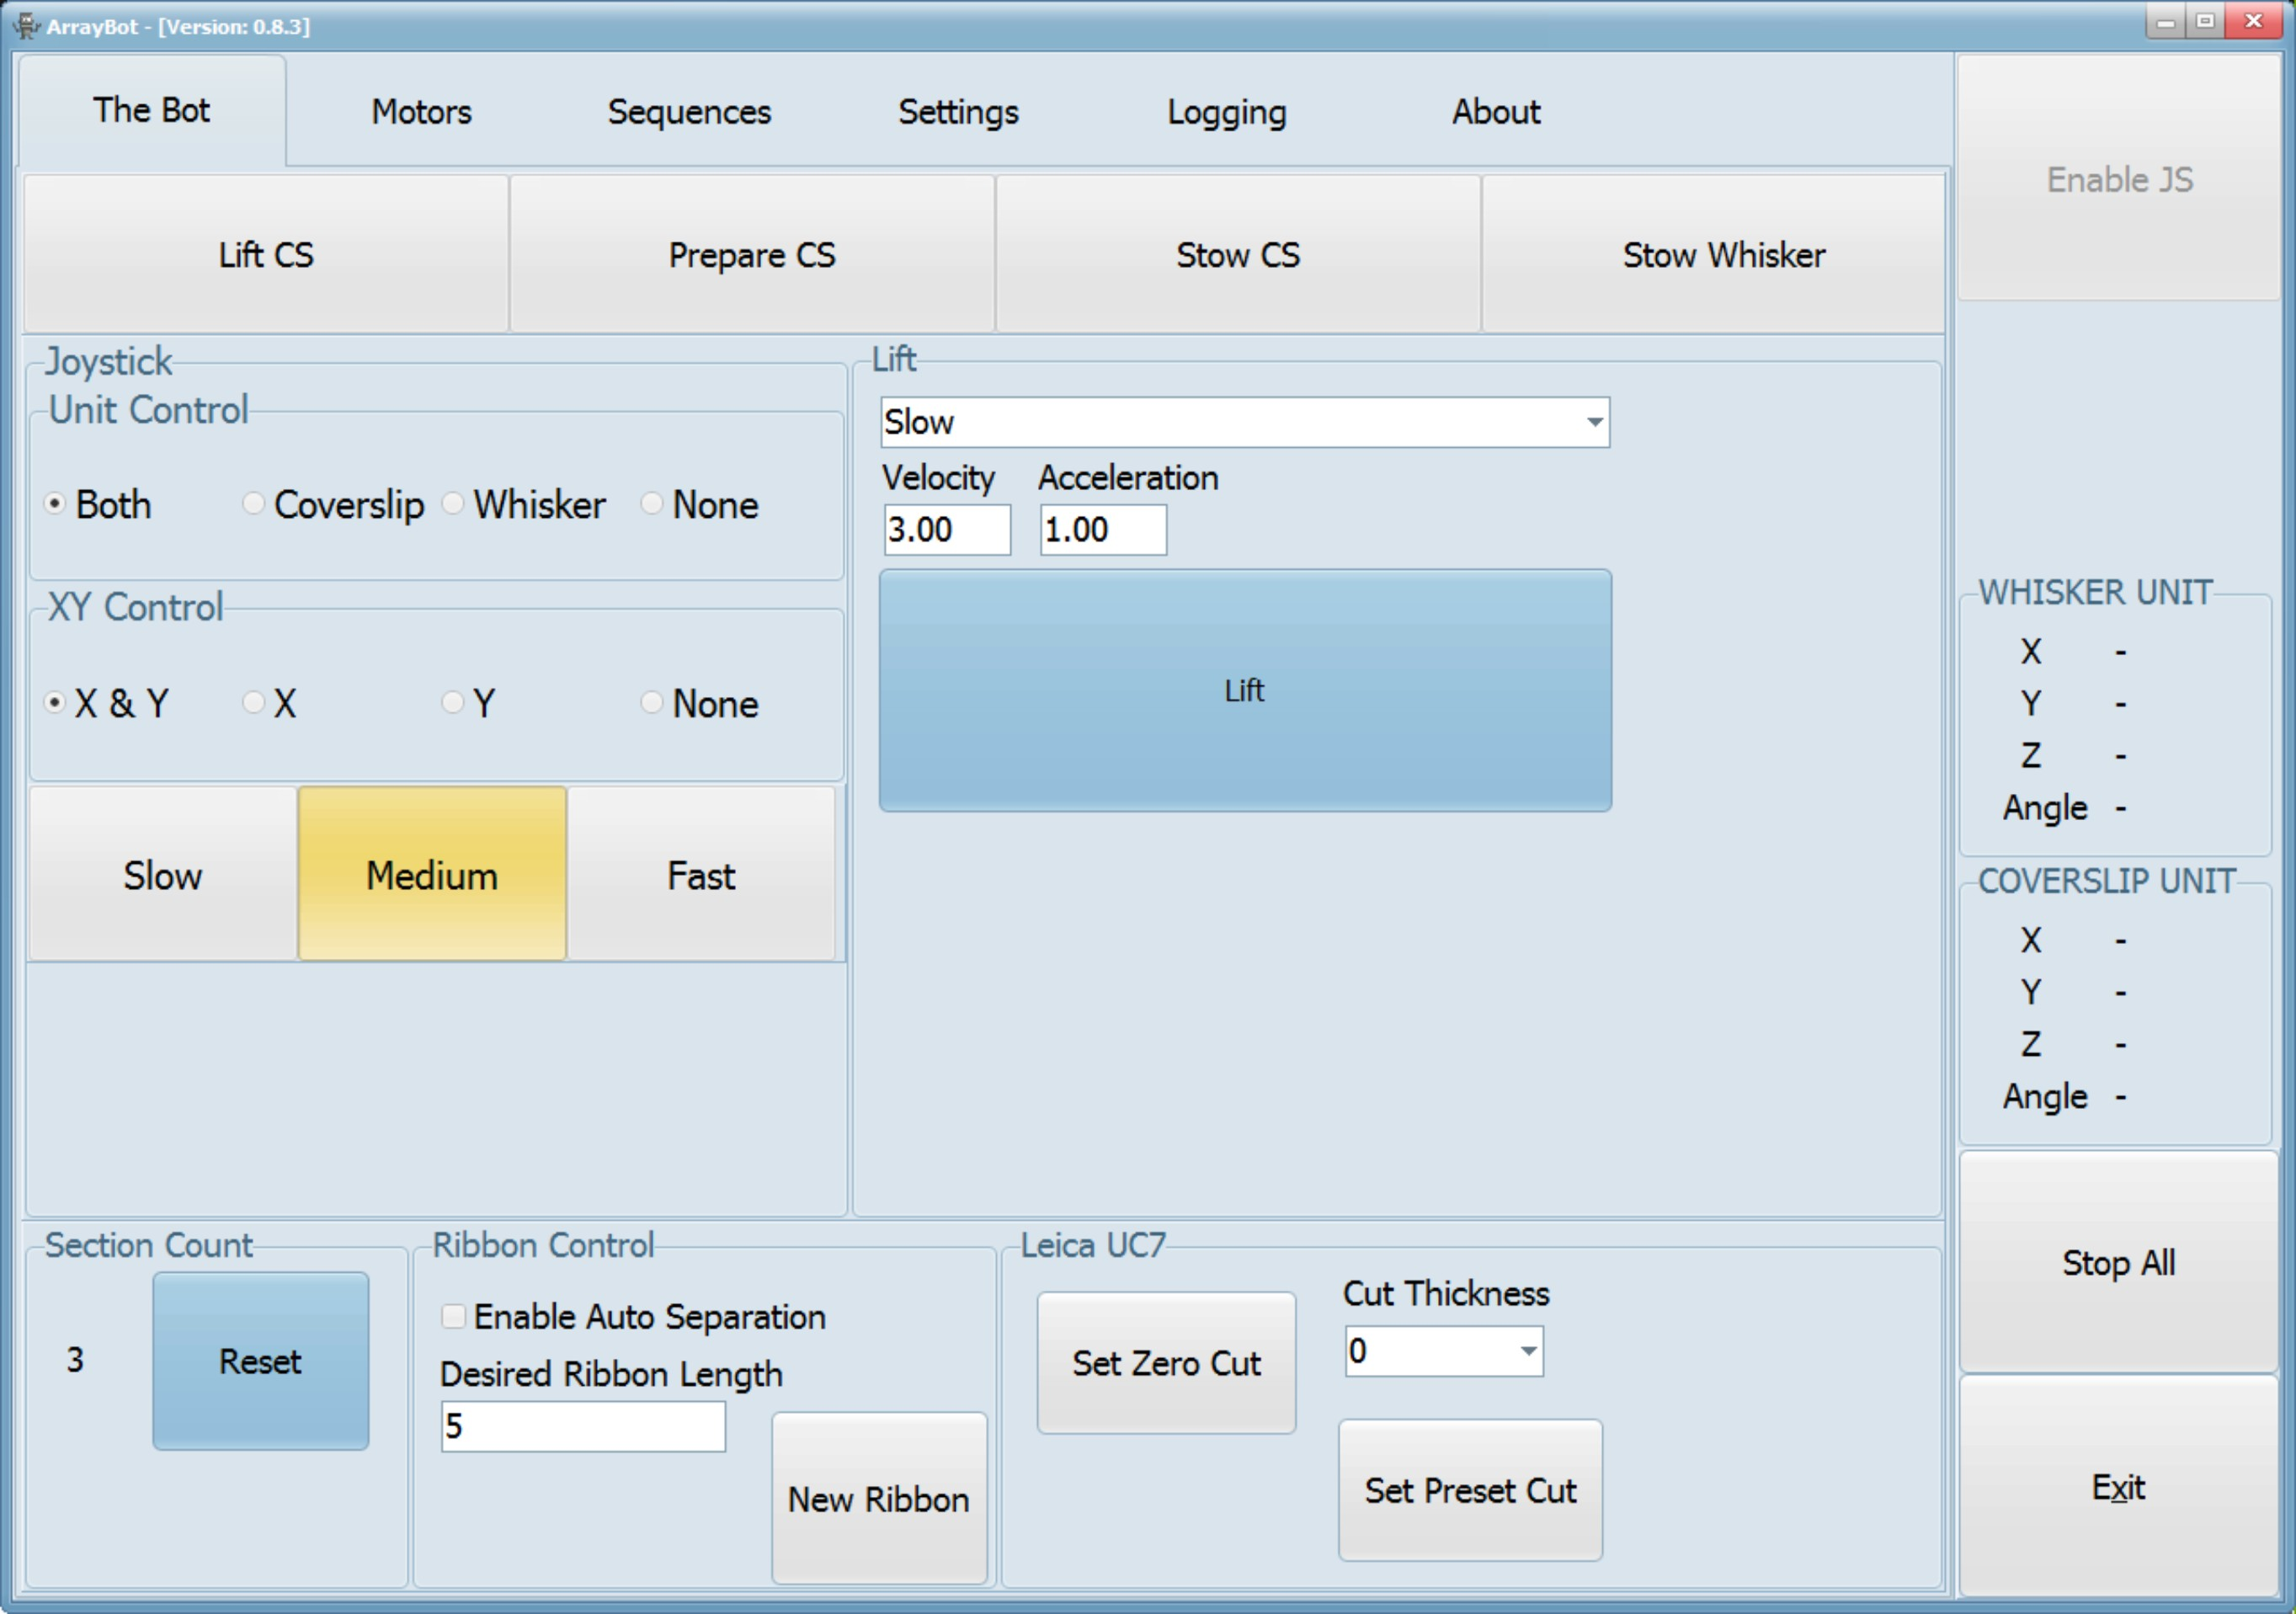
\includegraphics[scale=0.85]{AB_UI_1}
\caption{\ab{} UI}
\end{sidewaysfigure}

\clearpage

\subsection{\ac{} UI}

\begin{sidewaysfigure}[h]
\centering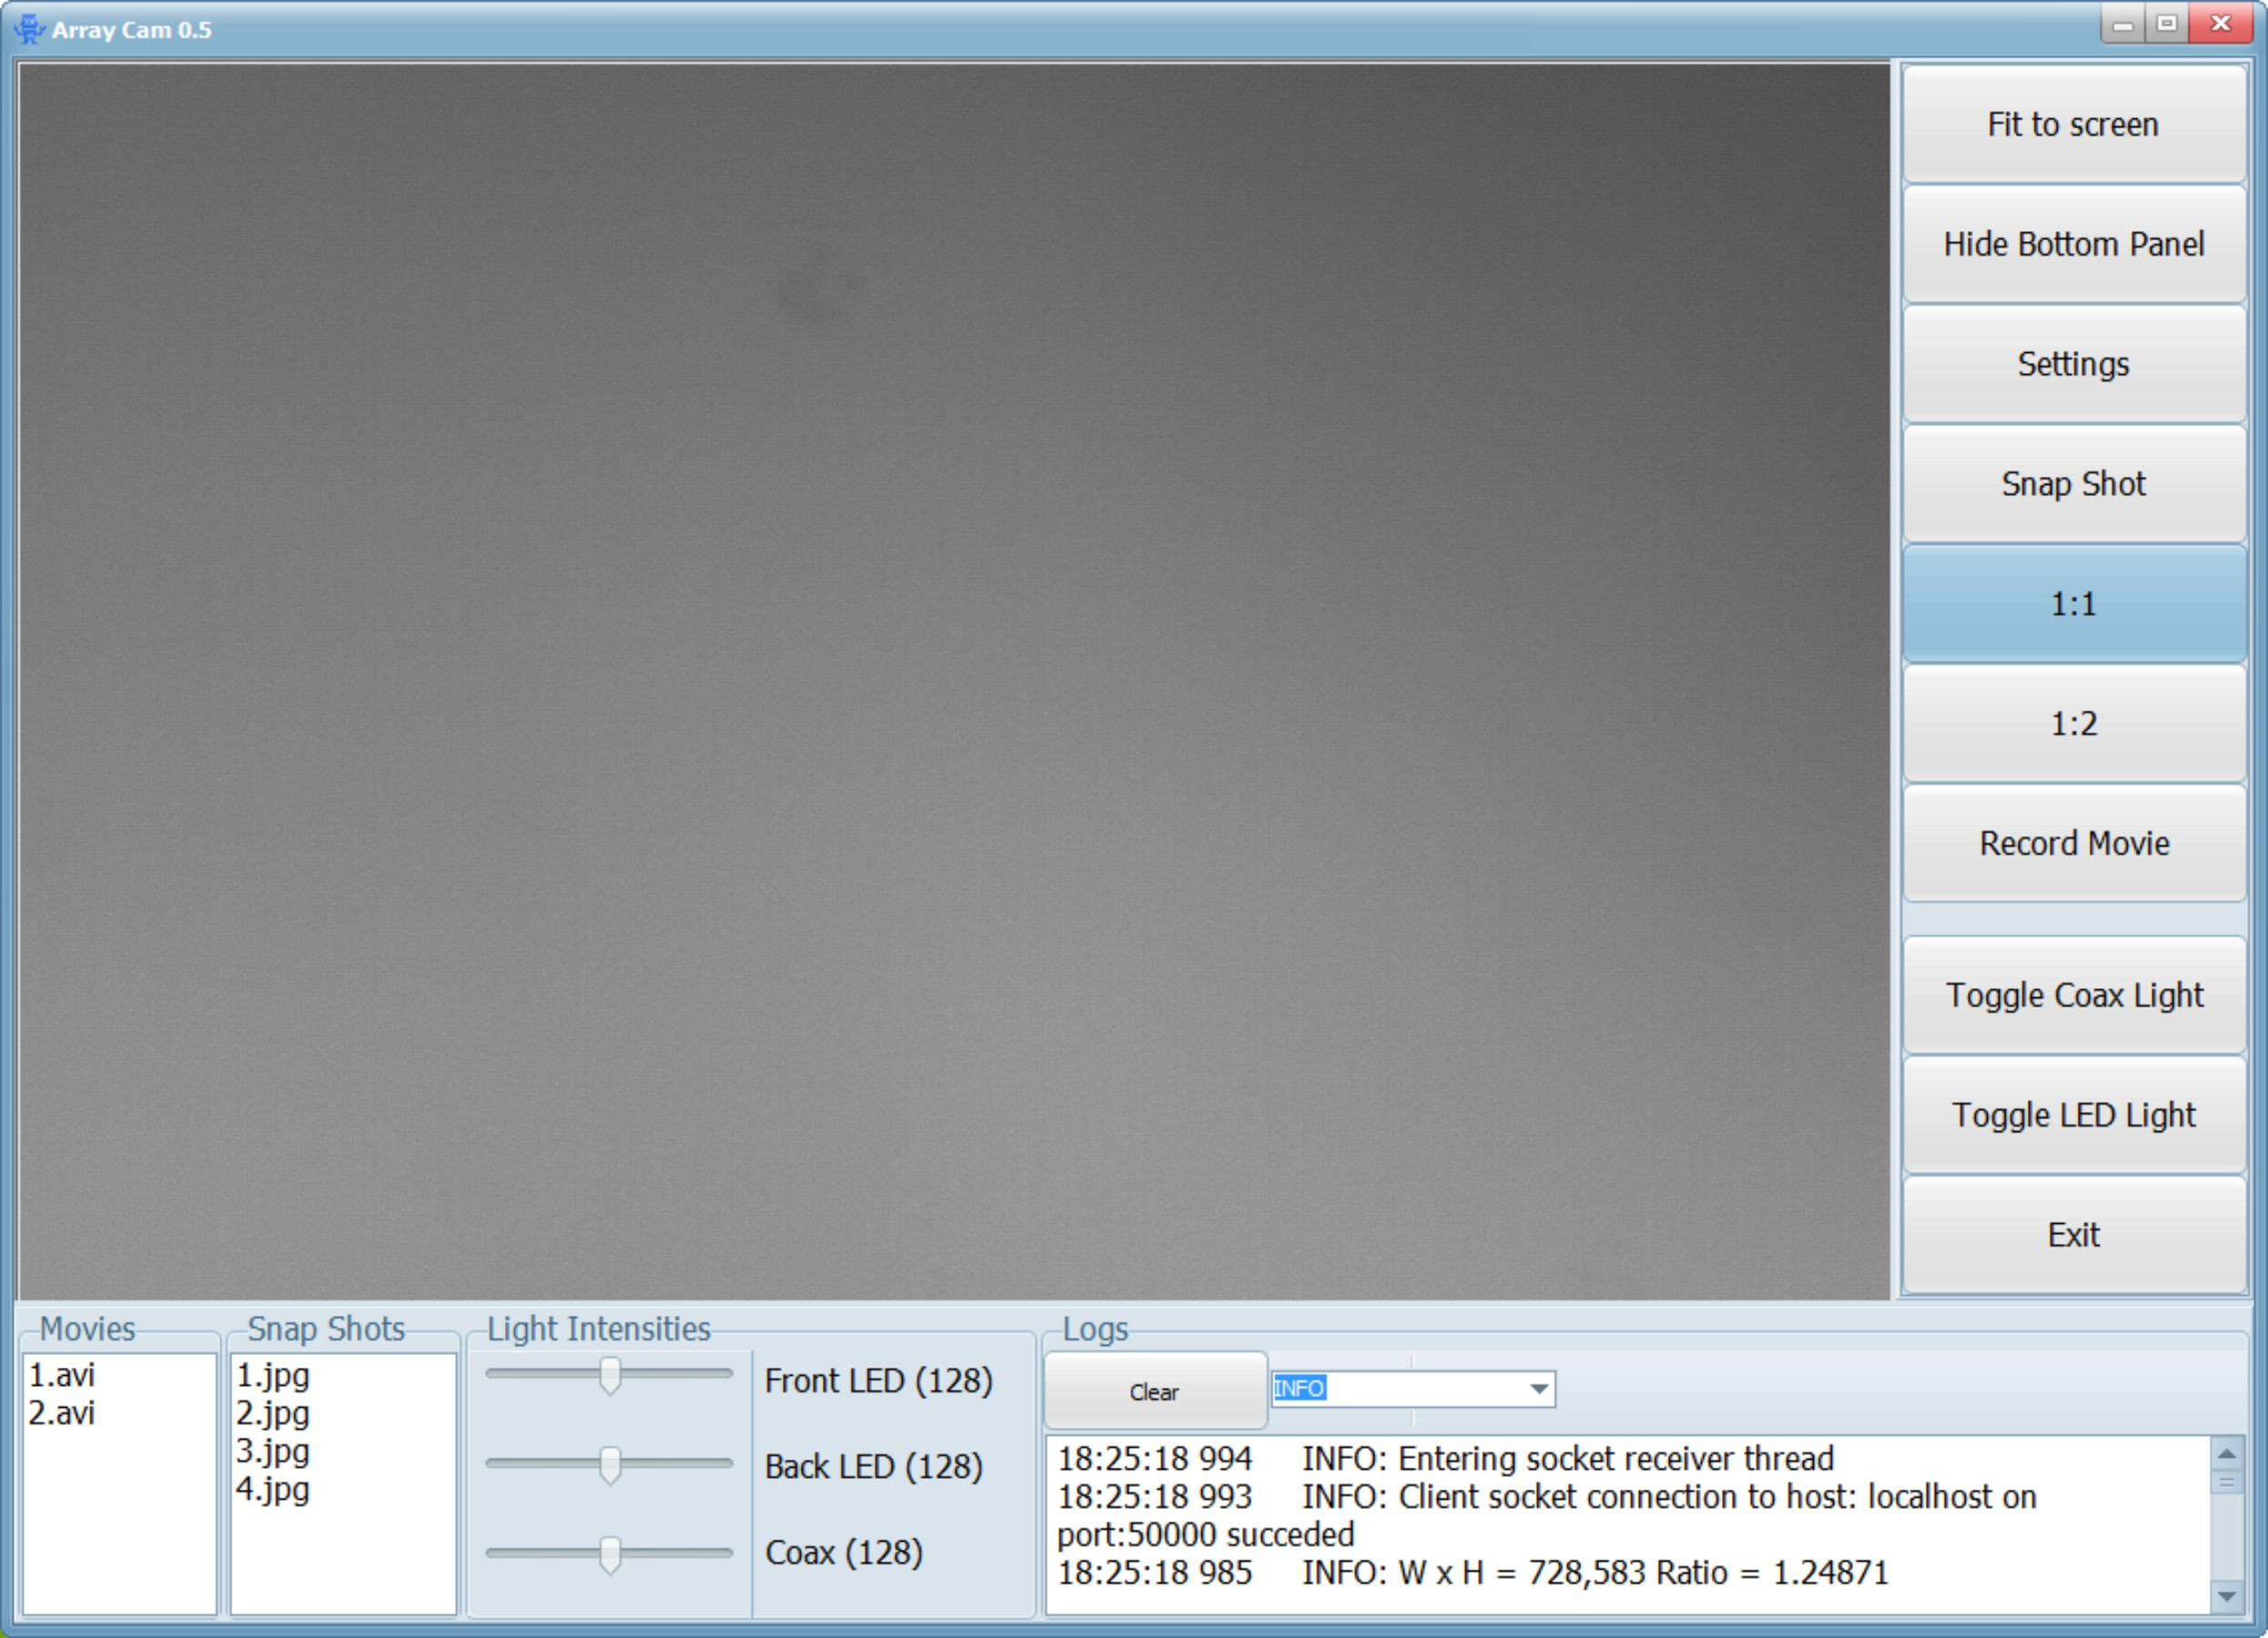
\includegraphics[scale=0.85]{AC_UI_1}
\caption{\ac{} UI}
\end{sidewaysfigure}

\clearpage
\subsection{\abc{} UI}
\begin{sidewaysfigure}[h]
\centering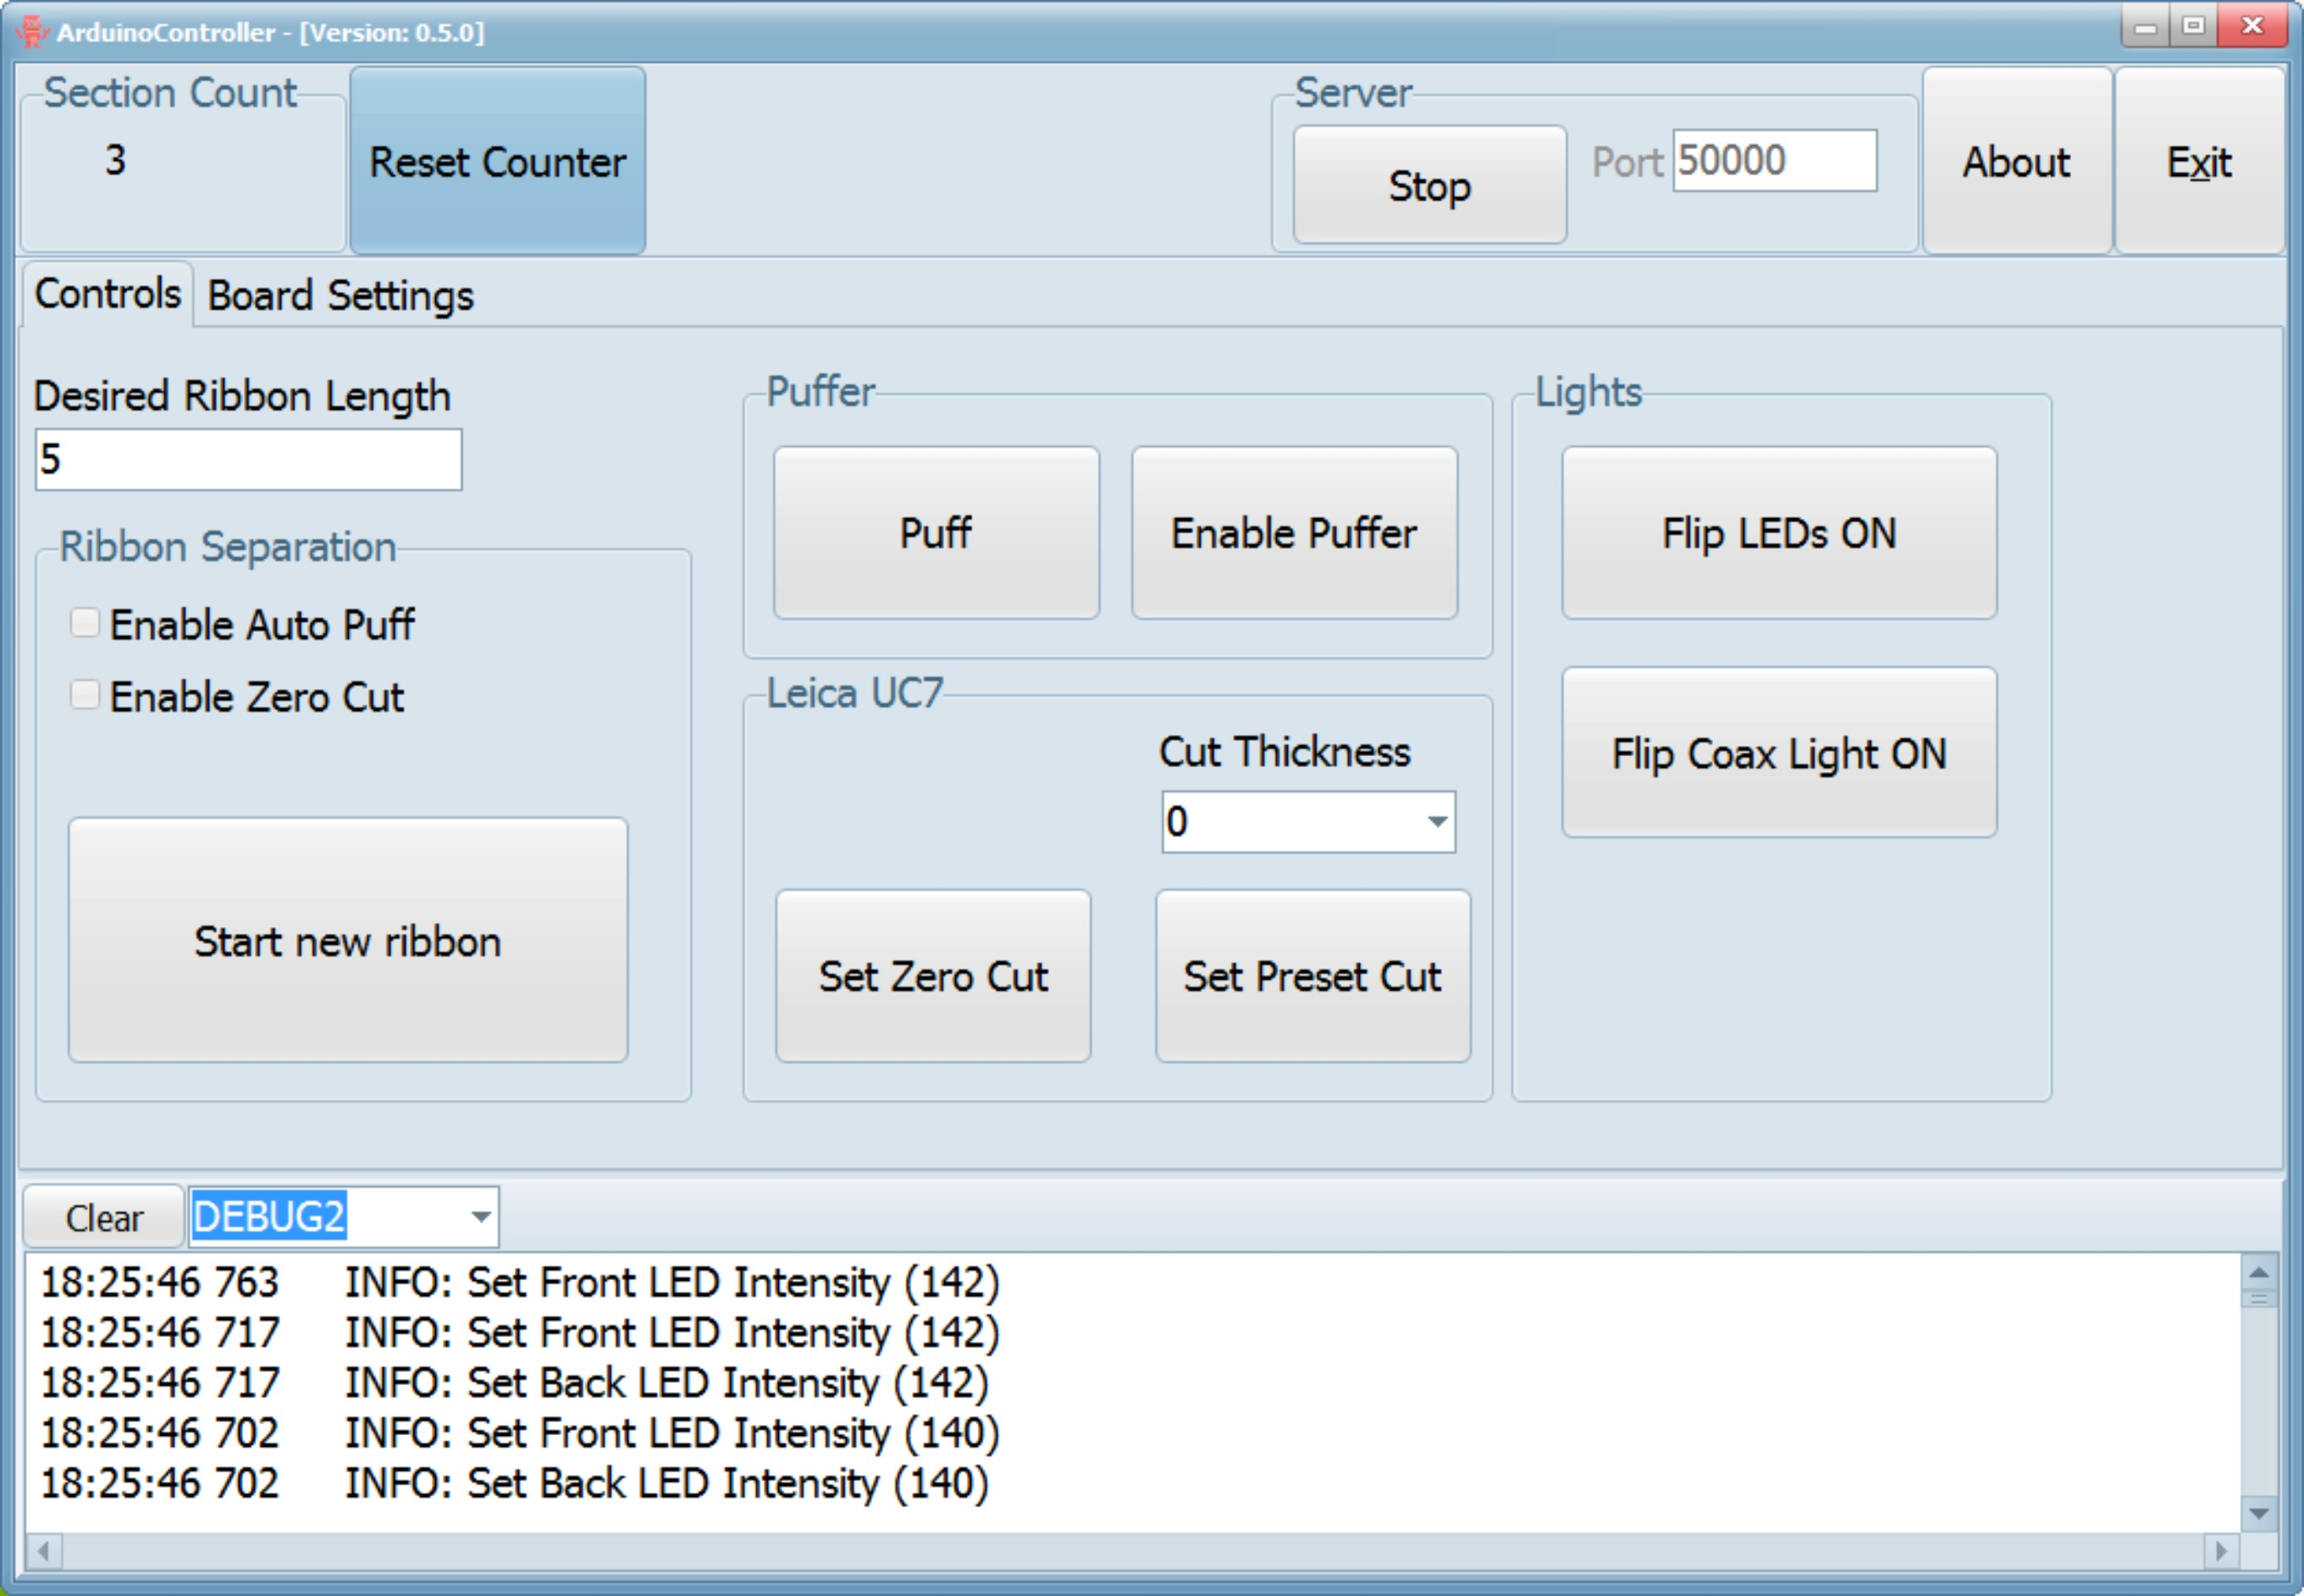
\includegraphics[scale=0.85]{ARDC_UI_1}
\caption{\abc{} UI}
\end{sidewaysfigure}

\clearpage


\section{Arraybot Hardware Setup}

\subsection{Motors}
\subsection{Arduinos}
\subsection{The Camera}


\chapterimage{ch_2.jpg} 


\chapter{Software Design and Software Components}

\section{Rough Software setup - picture}


\chapter{IPC}
\section{Serial Communication}
\section{The socket server and socket clients}

\chapter{Process Sequencer}
The process sequencer component is designed to allow the user to define and execute a sequence of various actions, e.g. moves.

\subsection{Process Sequence}
\subsection{Process	}
\subsection{XML}
\subsection{Triggers}

\chapter{The JoyStick}
\subsection{JoyStickMessageDispatcher}

\chapter{Controlling the motors}
\section{DeviceManager}
\section{APTDevice}
\subsection{APTMotor}
\subsection{LongTravelStage}
\subsection{TCube Stepper Motor}
\subsection{TCube DCServo}
\subsection{Angle Controller}
\section{XYZUnit}


\chapter{The Arduino Server}
The Arduino server class encapsulate Arduino peripherals in the Arraybot system, i.e. the sensor, puffer and the Leica Arduinos. Clients are served with Arduino related messages over a
TCP/IP socket.  

The Arduino server is a descendant of the IPC server class that is implementing all
network functionality.

The Arduino server forwards any messages sent from the arduino board to connected TCP/IP clients.

The purpose of each one of the three Arduinos, the Puffer board, the Sensor board and the Leica Arduino board, are discussed in sections below.

\section{Messages exchanged with the Arduino Server}
This section discusses the messaging protocol for the Arduino Server. The protocol is defined by a few simple text messages (short strings) that can be exchanged with the server. 

Typically a client sends (1) a command to the server, e.g. "ENABLE\_PUFFER", (2) the server receives and handles the message, possibly causing peripheral hardware to be modified, and (3) a response may be sent back to the client. 

The design emphasizes simplicity and so the error checking implemented in the system is held to a minimum. For example, a client sending a request do not typically implement a mechanism to handle a server response notifying if the request was carried out or not.
Instead, this system rely on careful debugging by the user, in reading error and warning log messages.


\subsection{Incoming messages}

Table \ref{tab:ima} lists commands that the \ar{} server accepts.
\begin{table}[h]
\centering
\begin{tabular}{l l  p{180pt}}
\toprule
\textbf{Text Message} & \textbf{Args} & \textbf{Description} \\
\midrule
RESET\_SECTION\_COUNT 	        & none & This message is a request to reset the current section count. \\
ENABLE\_PUFFER                  & none & Request to enable the puffer. \\  
DISABLE\_PUFFER                 & none & Request to disable the puffer. \\  
ENABLE\_AUTO\_PUFF              & none & Enable AutoPuff mechanims. \\  
DISABLE\_AUTO\_PUFF             & none & Disable AutoPuff mechanims. \\  
SET\_DESIRED\_RIBBON\_LENGTH    & none & Set desired ribbon length. Used when the AutoPuff mechanism is enabled. \\  
PUFF                            & none & Request a (manual) puff. \\  
START\_NEW\_RIBBON              & none & Request initiation of a new ribbon. This command will restore the current cut thickness preset and reset the section count. \\  
TURN\_ON\_LED\_LIGHTS				& -		& Turn on LED's \\
TURN\_OFF\_LED\_LIGHTS				& -		& Turn off LED's \\
TURN\_ON\_COAX\_LIGHTS				& -		& Turn on Coax lights \\
TURN\_OFF\_COAX\_LIGHTS			& -		& Turn on Coax lights \\
TOGGLE\_LED\_LIGHT              & none & Toggle LED light on/off. \\  
TOGGLE\_COAX\_LIGHT             & none & Toggle Coax light on/off. \\  

SET\_FRONTLED                   & none & Set Front LED intensity. \\  
SET\_BACKLED                    & none & Set Back LED intensity. \\  
SET\_COAX                       & none & Set Coax LED intensity. \\  
SET\_CUT\_PRESET                & none & Set cut thickness preset. \\  
SET\_DELTAY                     & none & Set mouse delta Y on the Leica UI. \\  
GET\_SENSOR\_ARDUINO\_STATUS       & none & Get general server status. \\  
SENSOR\_CUSTOM\_MESSAGE      		& none &  \\  
GET\_PUFFER\_ARDUINO\_STATUS       & none &  \\  
GET\_SERVER\_STATUS      			& none &  \\  

\bottomrule
\end{tabular}
\caption{Incoming messages handled by the Arduino server}\label{tab:ima}
\end{table}

\newpage

\subsection{Outgoing messages}
\begin{table}[h]
\centering
\begin{tabular}{l l p{160pt}}
\toprule
\textbf{Text Message} & \textbf{Initiated by} & \textbf{Description}\\
\midrule
GET\_READY\_FOR\_ZERO\_CUT\_1 	& Puffer Arduino & This message is sent two counts before a zero cut is to be executed. \\
GET\_READY\_FOR\_ZERO\_CUT\_2 	& Puffer Arduino & This message is sent one counts before a zero cut is to be executed. \\
SET\_ZERO\_CUT\_1 				& Puffer Arduino & This message is sent when a zero cut is to be executed. \\
RESTORE\_FROM\_ZERO\_CUT 		& Puffer Arduino & This message is sent after a zero cut. \\
\bottomrule
\end{tabular}
\caption{Arduino server response messages}\label{tab:asrm}
\end{table}


\newpage

\section{The Puffer and ribbon separation}
Individually cut sections are held together by a thin film of glue. The glue is part of the 'block-phase' and is necessary in order to successfully create a ribbon of consecutive tissue sections. However, the glue may also make a cut section stick to the knife itself.\\
In order to separate a ribbon from the knife, as to give way to a new ribbon, a mechanism involving an air puffer together with a zero thickness cut, allows for automatic separation of a ribbon from the knife.

The puffer mechanics is controlled by an Arduino, and the zero cut is controlled by serial communication between the Leica ultra-microtome and the host computer.


\subsection{Puffer Arduino Communication Protocol}
The Puffer Arduino hardware are connected to the ArrayBot software using a serial (COM) port. This allow messaging between the PC software and  the Arduino Software. 

The Puffer Arduino implements a simple messaging protocol, involving receive/transmit of a few bytes over the serial port connection.

Table \ref{tab:pac} lists the commands that are currently implemented in the Puffer Arduino Software.

\begin{table}[h]
\centering
\begin{tabular}{l l p{160pt} p{160pt}}
\toprule
\textbf{Command} & \textbf{Arguments} & \textbf{Usage} & \textbf{Note}\\
\midrule
S	& 1 or 0	& Enable/Disable simulation of the Hall Sensor. & For debugging purposes. \\
s	& int		& Set simulation speed. The supplied integer denotes the delay, in ms, between sending simulated Hall sensor switch messages. & For debugging purposes. \\
P	& int	& Set cut thickness preset on the Leica. &  This command results in a request to the Leica Arduino to change the cut thickness preset. Valid values are 1-5\\
Y	& int	& Set deltaY for mouse movement on the Leica. &  \\
e	&   & Enable the puffer &  \\
a	&   & Disable the puffer &  \\
p	&   & Request an immediate puff &  \\
d	& int   & Set puff duration in ms &  \\
v	& int   & Set puff valve speed. Valid values are 0-255. &  \\
i	& int   & Request info about current Arduino state. &  \\
\bottomrule
\end{tabular}
\caption{Puffer Arduino commands}\label{tab:pac}
\end{table}

\begin{table}[h]
\centering
\begin{tabular}{l p{160pt} p{80pt}}
\toprule
\textbf{Message} & \textbf{Usage} & \textbf{Note}\\
\midrule
LEICA MESSAGE: "..." 			& Forwarded message from the Leica Arduino & For debugging. \\
HALL\_SENSOR='VALUE' 			& Message indicating the value of the Hall Sensor. VAL = HIGH or LOW & \\
REQUEST\_CUT\_PRESET\_'VALUE' 	& Indicating we are requesting to change the cut thickness preset on the Leica. VAL = 1-5 & \\
CUT\_PRESET\_VALUE IS INVALID 	& Error response &\\
REQUEST\_DELTA\_Y='VALUE'   	& Indicating request to change the delta Y value on the Leica. VAL = any integer & \\
PUFFER\_ENABLED					& Indicate that the puffer was enabled & \\
PUFFER\_DISABLED				& Indicate that the puffer was disabled & \\
EXECUTED\_PUFF 					& Puffer was executed & \\

\bottomrule
\end{tabular}
\caption{Puffer Arduino Client Messages}
\end{table}


\section{Sensors and Lights}
Lights and sensors are read/controlled by a third Arduino - the 'Sensor' Arduino.


Table \ref{tab:sac} lists the commands that are currently implemented in the Sensor Arduino Software.

\begin{table}[h]
\centering
\begin{tabular}{l l p{160pt} p{160pt}}
\toprule
\textbf{Command} & \textbf{Arguments} & \textbf{Usage} & \textbf{Note}\\
\midrule
1		& -	& Button1 Down & Turn on light? \\
2		& -	&  Down &  				\\
3		& -	&  Down & \\
3		& -	&  Down & \\
4		& -	&  Down & \\
5		& -	&  Down & \\
c		& int	&  Set coax drive 0-255 & \\
f		& int	&  Set front LED drive 0-255 & \\
b		& int	&  Set back LED drive 0-255 & \\
i		& 	&  Return information about states & \\

\bottomrule
\end{tabular}
\caption{Sensor Arduino Commands}\label{tab:sac}
\end{table}

\begin{table}[h]
\centering
\begin{tabular}{l l p{160pt} p{160pt}}
\toprule
\textbf{Response} & \textbf{Description}\\
\midrule
BUTTON\_1\_DOWN & Turn off Coax LEDS \\
BUTTON\_2\_DOWN &  \\
BUTTON\_3\_DOWN &  \\
BUTTON\_4\_DOWN &  \\
BUTTON\_5\_DOWN &  \\
COAX\_DRIVE=		&	\\
FRONT\_LED\_DRIVE=		&	\\
BACK\_LED\_DRIVE=		&	\\
PIN\_1\_DOWN			&	\\
DHT22\_DATA=			& \\
DHT22\_ERROR & \\


\bottomrule
\end{tabular}
\caption{Sensor Arduino Responses}\label{tab:sac}
\end{table}

\clearpage

\section{Hardware Setup}
\subsection{Arduino setup}
The figure and tables below discusses the hardware setup of the three Arduinos, the PC and the leica microtome

\begin{figure}[h]
\centering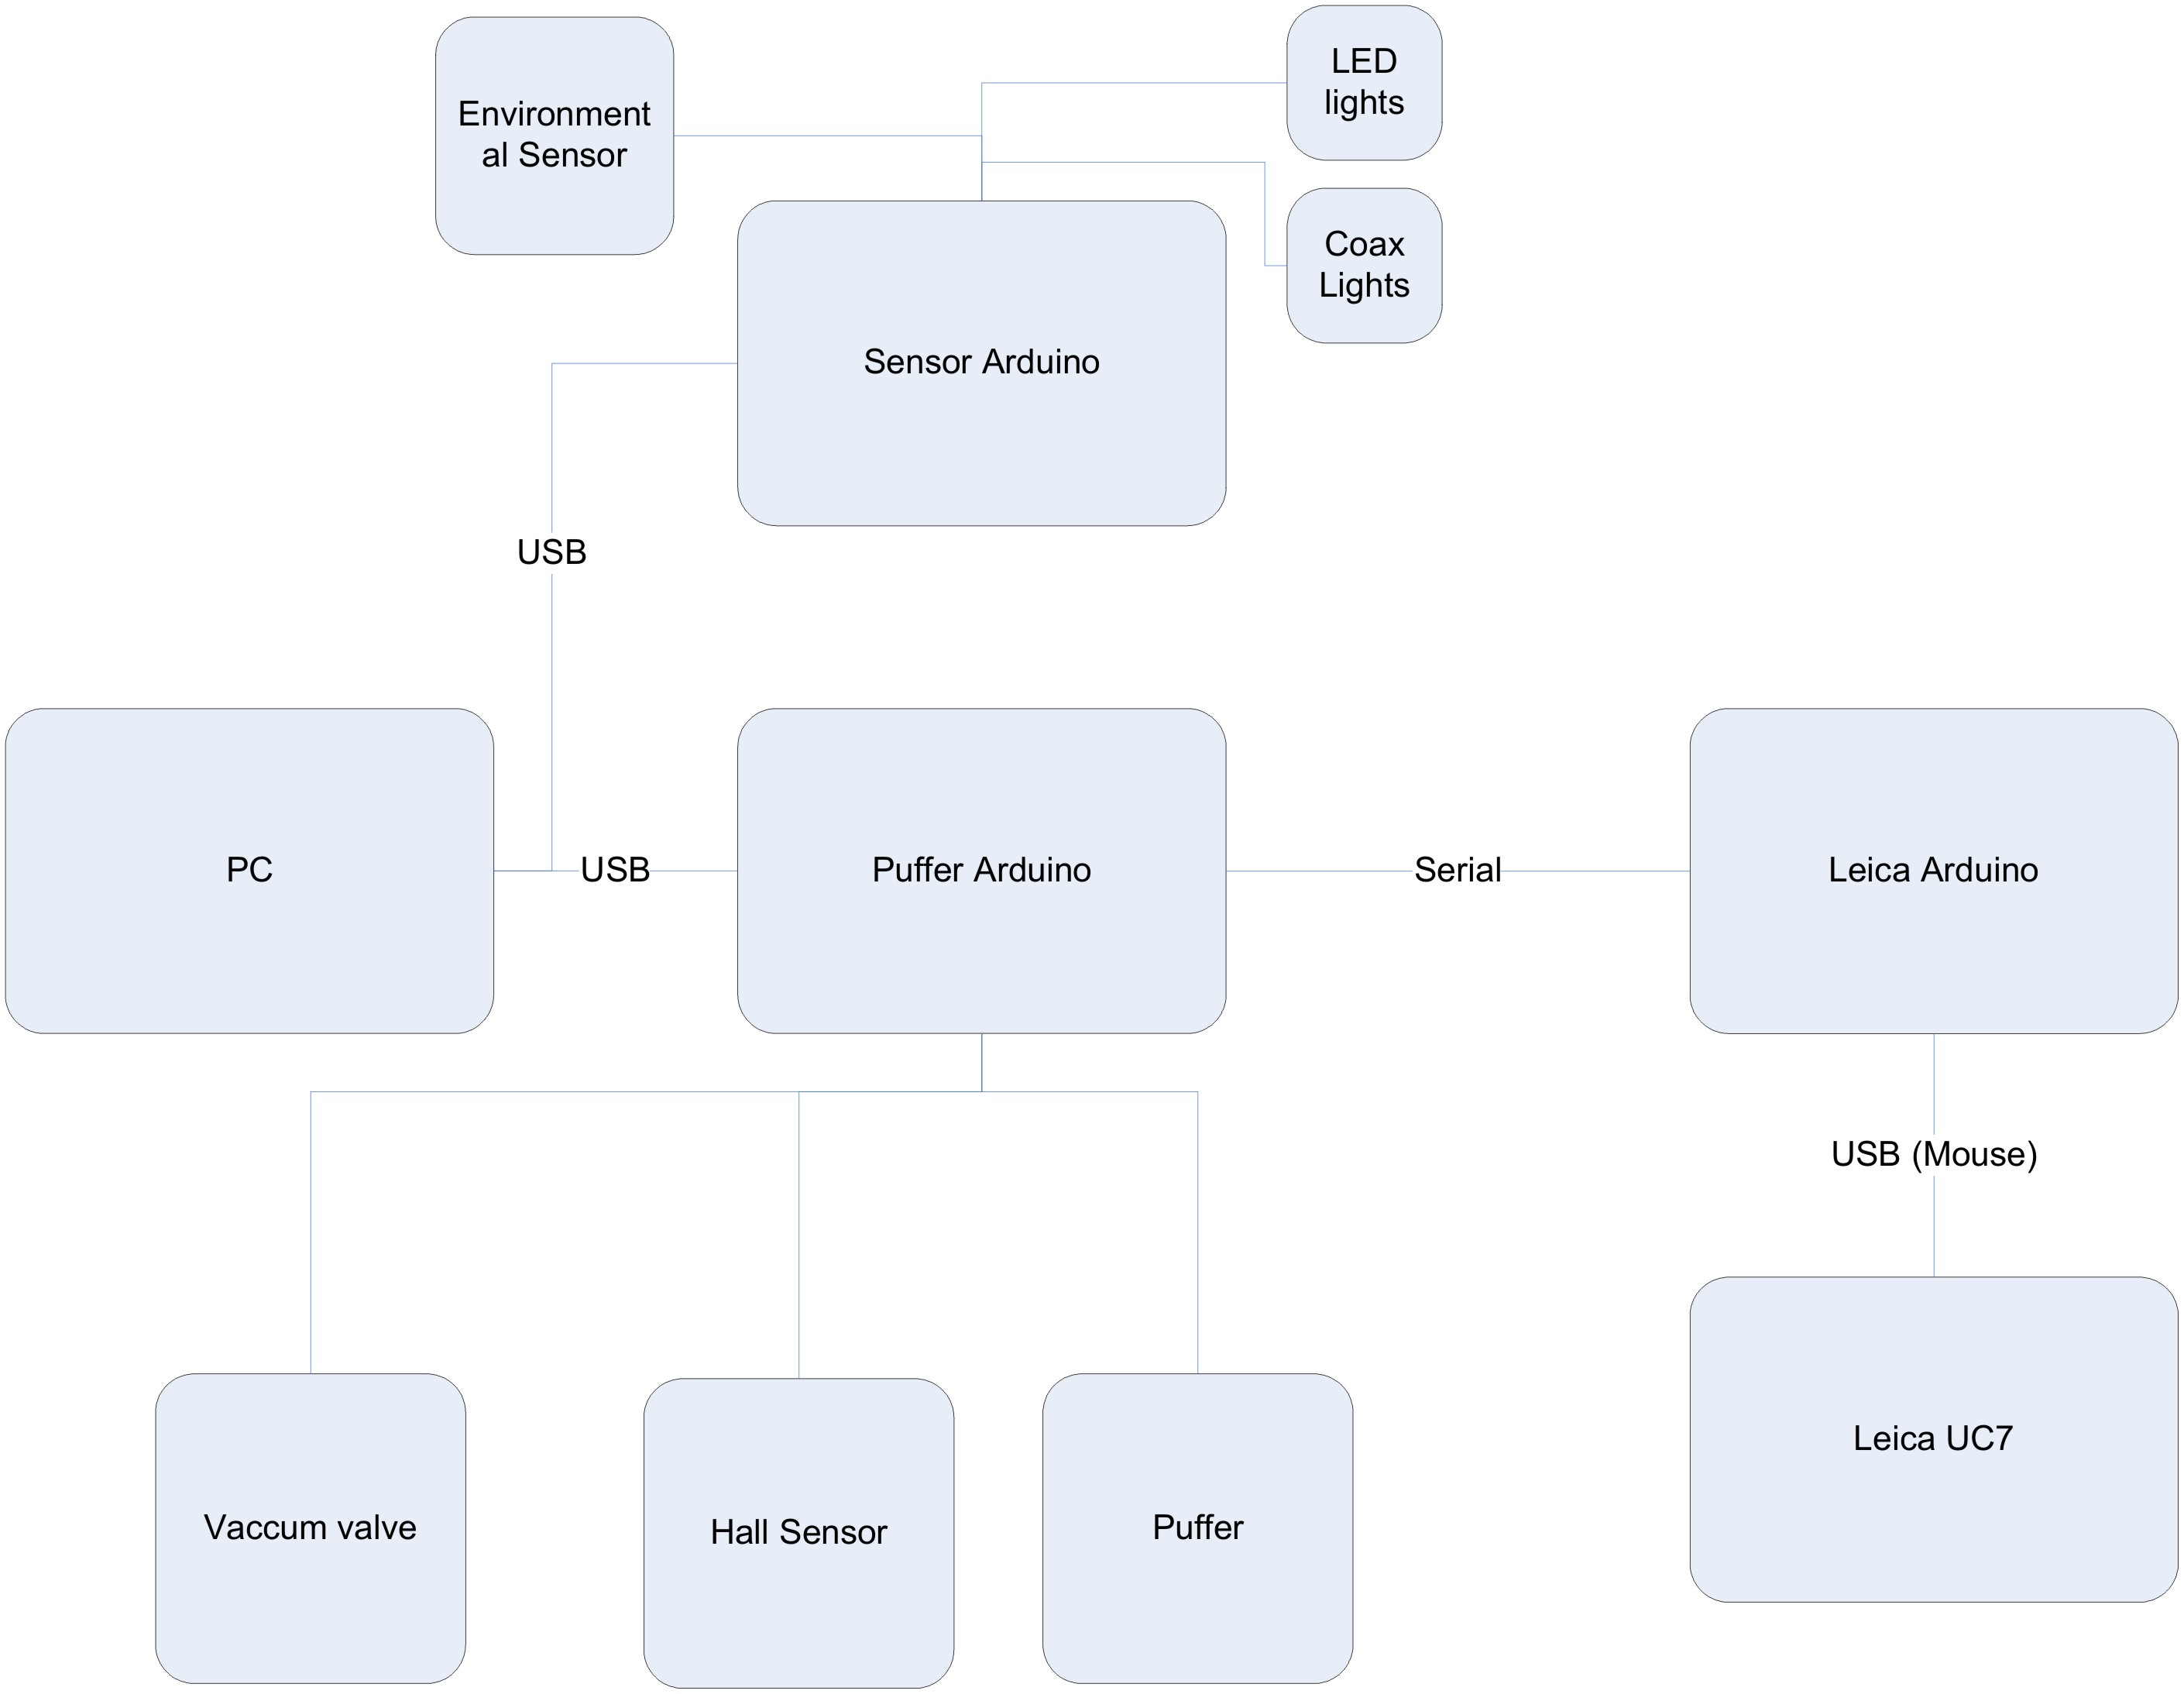
\includegraphics[scale=0.5]{arduino_hw_setup}
\caption{Arduino hardware setup}
\end{figure}




\begin{appendices}
\chapter{Get the source code}

Public Software Repository: $\mathbf{git@github.com:TotteKarlsson/ArrayBot.git}$

\chapter{Software API's}

\section{ArrayBot Software API's}\index{ArrayBot Software API's}
\subsection{abCore}
\subsection{abVCLCore}

\section{ThirdParty libraries}
\subsection{Poco}
\subsection{libcurl}
\subsection{SQLite}
\subsection{tinyxml2}
\subsection{uc480 and uc480\_tools}
\subsection{Dune Scientific's libraries: mtkCommon, mtkMath, mtkIPC and mtkVCL}

\clearpage

\chapter{Arduino wiring}
\begin{table}[h]
\centering
\begin{tabular}{l l p{160pt}}
\toprule
\textbf{Pin \#} & \textbf{Usage} & \textbf{Note}\\
\midrule
0 	& Serial Receive 	& Used for serial communication \\
1 	& Serial Transmit  	& Used for serial communication \\
2 	& Hall Sensor 		&  \\
3 	& Puffer			&  \\
4 	&  &  \\
5 	&  &  \\
6 	&  &  \\
7 	&  &  \\
8 	&  &  \\
9 	&  &  \\
10 	& Serial Receive  & Connection to the Leica Arduino Serial port \\
11 	& Serial Transmit & Connection to the Leica Arduino Serial port \\
12 	&  &  \\
13 	& LED Illuminates when Hall sensor is high &  \\
\bottomrule
\end{tabular}
\caption{Puffer Arduino Pins}\label{tab:pap}
\end{table}



\begin{table}[h]
\centering
\begin{tabular}{l l p{160pt}}
\toprule
\textbf{Pin \#} & \textbf{Usage} & \textbf{Note}\\
\midrule
0 	& Serial Receive 	& Used for serial communication \\
1 	& Serial Transmit  	& Used for serial communication \\

\bottomrule
\end{tabular}
\caption{Sensor Arduino Pins}
\end{table}


\begin{table}[h]
\centering
\begin{tabular}{l l p{160pt}}
\toprule
\textbf{Pin \#} & \textbf{Usage} & \textbf{Note}\\
\midrule
0 	& Serial Receive 	& Used for serial communication to Puffer Arduino\\
1 	& Serial Transmit  	& Used for serial communication to Puffer Arduino\\
2 	& unused &  \\
3 	& unused &  \\
4 	& unused &  \\
5 	& unused &  \\
6 	& unused &  \\
7 	& unused &  \\
8 	& unused &  \\
9 	& unused &  \\
10 	& unused & \\
11 	& unused &\\
12 	& unused &  \\
13 	& unused &  \\
\bottomrule
\end{tabular}
\caption{Leica Arduino Pins}
\end{table}

\clearpage

\end{appendices}




%%----------------------------------------------------------------------------------------
%%	BIBLIOGRAPHY
%%----------------------------------------------------------------------------------------
%\chapter*{Bibliography}
%\addcontentsline{toc}{chapter}{\textcolor{ocre}{Bibliography}}
%\section*{Books}
%\addcontentsline{toc}{section}{Books}
%\printbibliography[heading=bibempty,type=book]
%\section*{Articles}
%\addcontentsline{toc}{section}{Articles}
%\printbibliography[heading=bibempty,type=article]
%
%%----------------------------------------------------------------------------------------
%%	INDEX
%%----------------------------------------------------------------------------------------
%
%\cleardoublepage
%\phantomsection
%\setlength{\columnsep}{0.75cm}
%\addcontentsline{toc}{chapter}{\textcolor{ocre}{Index}}
%\printindex
%
%%----------------------------------------------------------------------------------------
%
\end{document}
